\documentclass[11pt,a4paper]{article}
\usepackage[utf8]{inputenc}
\usepackage{amsmath, amssymb, amsthm}
\usepackage{geometry}
\usepackage{graphicx}
\usepackage{booktabs}
\usepackage{hyperref}
\usepackage{xcolor}
\usepackage{empheq}

\geometry{margin=1in}

\title{\textbf{Information Theory}}
\author{\textbf{Nishanka Das} \\ 
Department of Computer Science \\ 
Ramakrishna Mission Vivekananda Centenary College, Rahara}
\date{\today}

\begin{document}

\maketitle

\begin{center}
For any mistakes found please feel free to mail at: \\
\url{nishanka.das.rkmvcc@gmail.com}
\end{center}

\begin{abstract}
This document provides a rigorous, self-contained exploration of foundational information theory and its structural intersection with statistical mechanics and continuous probability spaces. We begin by establishing Claude Shannon's core framework, detailing how the qualitative measure of information scales inversely with probability as a metric of structural surprise, and formalizing the discrete formulation of Shannon entropy. We provide a geometric analysis of the binary entropy function to demonstrate how uncertainty peaks within a uniform discrete system. Moving from information to physics, we construct the thermodynamic bridge linking macrostate multiplicity with Shannon uncertainty using Stirling's asymptotic approximation. Using variational calculus with a single Lagrange multiplier, we formally prove why a discrete uniform distribution maximizes entropy under basic normalization constraints. The framework is then extended to continuous variables by applying the Mean Value Theorem for Integrals to derive differential entropy from a limiting quantization scheme. Finally, we utilize multi-constraint functional optimization to demonstrate that the Gaussian distribution represents the state of maximum continuous chaos under a fixed mean and variance, and introduce relative metrics including the Kullback-Leibler divergence, conditional entropy, and mutual information.
\end{abstract}
\section{Entropy}
Information theory provides the essential mathematical framework for quantifying uncertainty, data compression, and transmission efficiency, making it an indispensable pillar for designing loss functions and probabilistic frameworks in machine learning. At the absolute core of this theory lies the concept of entropy.

\subsection{Information Content as a Measure of Surprise}
Before formalizing a macro-level metric, we must define what information represents at the level of an individual outcome. Mechanistically, the information content of an event is directly proportional to its degree of \textit{surprise} or improbability:
\begin{itemize}
    \item \textbf{High Probability $\implies$ Low Surprise:} An event with a probability approaching $1$ (e.g., ``the sun will set tonight'') yields virtually zero new information because its occurrence was already an absolute certainty.
    \item \textbf{Low Probability $\implies$ High Surprise:} An event with a low prior probability (e.g., ``an earthquake is occurring at these exact coordinates'') yields an immense cascade of information because it radically restructures an observer's state of knowledge.
\end{itemize}

Let $x$ be a specific realization of a discrete random variable $X$ governed by a probability mass function $p(x)$. To design a mathematically robust function $h(x)$ capable of measuring this surprise, it must satisfy three axiomatic constraints:
\begin{enumerate}
    \item \textbf{Monotonicity:} The informational value must scale inversely with probability: $p(x_1) > p(x_2) \implies h(x_1) < h(x_2)$.
    \item \textbf{Boundary Condition:} An event with absolute certainty carries exactly zero informational value: $p(x) = 1 \implies h(x) = 0$.
    \item \textbf{Additivity:} The total information gained from observing two mutually independent events $x$ and $y$ must equal the sum of their individual surprises: $h(x, y) = h(x) + h(y)$.
\end{enumerate}

Given that the events are statistically independent, their joint probability is multiplicative: $p(x, y) = p(x) \cdot p(y)$. The logarithm is uniquely capable of mapping a product of continuous variables into a linear sum of scalar values ($\ln(A \cdot B) = \ln A + \ln B$). Accounting for the boundary constraint where $p(x) \le 1$, we define the information content of a single outcome as:
\begin{equation}
h(x) = -\ln p(x)
\end{equation}

\subsection{The Mathematical Definition of Entropy}
While $h(x)$ quantifies the surprise of an isolated, discrete event, the \textbf{Shannon Entropy}, denoted $H(X)$, represents the mathematical expectation (or weighted average) of the informational surprise evaluated across all possible realizations of the system. 

For a discrete random variable $X$ taking values in the alphabet set $\{x_1, x_2, \dots, x_n\}$, its entropy is defined as:
\begin{equation}
H(X) = E[h(x)] = -\sum_{i=1}^{n} p(x_i) \log p(x_i)
\end{equation}

The qualitative units of uncertainty are governed strictly by the choice of the logarithmic base:
\begin{itemize}
    \item \textbf{Base 2 ($\log_2$):} Measures entropy in \textit{bits} (or shannons). This framework represents the average minimum number of binary (yes/no) questions required to fully determine the active state of $X$.
    \item \textbf{Natural Log ($\ln$):} Measures entropy in \textit{nats}. This base is highly preferred across physics, optimization calculus, and deep learning algorithms due to its elegant derivative properties.
\end{itemize}
\textit{Analytical Note:} By standard convention, if a certain state possesses an empirical probability of $p(x_i) = 0$, we evaluate the expression via its limit behavior: $\lim_{p \to 0} p \log p = 0$. Thus, impossible events safely drop out of the summation without destabilizing the system.

\subsection{Geometric Analysis: The Binary Entropy Function}
To visualize entropy strictly as a metric of structural uncertainty, consider a binary system—such as a biased coin flip—where the probability of a success outcome is given by $p$, and the failure outcome is $1-p$. The general equation collapses down to a single independent variable parameter:
\begin{equation}
H(X) = -p \log_2 p - (1-p) \log_2 (1-p)
\end{equation}

Tracing this function across its full probability domain ($0 \le p \le 1$) reveals a completely concave parabolic curve, as illustrated in Figure~\ref{fig:binary_entropy}.

\begin{figure}[htbp]
    \centering
    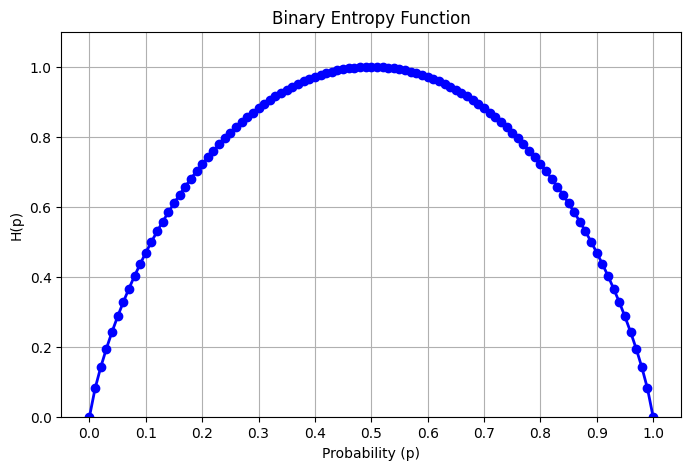
\includegraphics[width=0.7\textwidth]{demo.png}
    \caption{The Binary Entropy Function plotted across the probability domain, demonstrating the relationship between structural uncertainty and informational bits. The code can be found at \url{https://github.com/NishankaDas/ML-DL/blob/main/ML&DL/binary_cross_entropy.ipynb}}
    \label{fig:binary_entropy}
\end{figure}

Analyzing the critical geometric inflection points along this curve yields profound insights into uncertainty behavior:
\begin{itemize}
    \item \textbf{Absolute Certainty ($p = 1$ or $p = 0$):} At the boundaries, the system is entirely deterministic. Because you possess complete knowledge of the outcome prior to execution, the calculation drops to a minimum:
    \begin{equation}
    H(X) = -1\log_2(1) - 0\log_2(0) = 0 \text{ bits}
    \end{equation}
    Zero structural uncertainty yields zero entropy.
    \item \textbf{Highly Biased Distribution ($p = 0.9$):} The system remains heavily predictable, yet a minor fraction of surprise persists:
    \begin{equation}
    H(X) = -0.9\log_2(0.9) - 0.1\log_2(0.1) \approx 0.47 \text{ bits}
    \end{equation}
    \item \textbf{Maximum Uncertainty ($p = 0.5$):} The system represents a perfectly fair coin. There is absolutely no structural or statistical reason to favor one state over another. 
    \begin{equation}
    H(X) = -0.5\log_2(0.5) - 0.5\log_2(0.5) = 1 \text{ bit}
    \end{equation}
    This point forms the absolute global maximum peak of the curve. It formally demonstrates that a uniform distribution over states provides the maximum possible entropy for a discrete system.
\end{itemize}
\section{The Physics Perspective}
The definition of entropy originated in 19th-century thermodynamics through the work of Ludwig Boltzmann and Willard Gibbs, long before its informational adaptation by Claude Shannon.

\subsection{Microstates and Macrostates}
Consider a physical system defined at two distinct scales:
\begin{itemize}
    \item \textbf{Macrostate:} The large-scale macroscopic characteristics of a system, such as volume, pressure, and temperature.
    \item \textbf{Microstate:} A hyper-specific, exact spatial and kinematic arrangement of every constituent particle in the system.
\end{itemize}

\subsection{Deriving Entropy from Bin Multiplicity}
To bridge the physical configuration of space with informational uncertainty, let us consider a system containing $N$ total identical objects allocated across a set of discrete bins, where each $i$-th bin contains $n_i$ objects. The total capacity constraint yields:
\begin{equation}
\sum_{i} n_i = N
\end{equation}

The total number of unique arrangements—defined as the system's \textbf{multiplicity} ($W$), or the weight of the macrostate—is given by dividing total permutations by internal bin permutations:
\begin{equation}
W = \frac{N!}{\prod_{i} n_i!}
\end{equation}

We define the normalized physical entropy $H$ as the logarithm of this total configuration space scaled inversely by the total mass scale $1/N$:
\begin{equation}
H = \frac{1}{N} \ln W = \frac{1}{N} \ln \left( \frac{N!}{\prod_{i} n_i!} \right)
\end{equation}
Expanding using standard logarithmic rules converts the product operator into a discrete summation:
\begin{equation}
H = \frac{1}{N} \ln N! - \frac{1}{N} \sum_{i} \ln n_i!
\end{equation}

\subsection{Application of Stirling's Approximation}
To evaluate the asymptotic behavior of the system as the number of elements approaches infinity ($N \to \infty$), we apply \textbf{Stirling's Approximation} ($\ln N! \simeq N \ln N - N$) to both factorial terms:
\begin{align}
H &\simeq \frac{1}{N} (N \ln N - N) - \frac{1}{N} \sum_{i} (n_i \ln n_i - n_i) \\
H &\simeq (\ln N - 1) - \frac{1}{N} \sum_{i} n_i \ln n_i + \frac{1}{N} \sum_{i} n_i
\end{align}
Recalling that $\sum_{i} n_i = N$, the final scaling term simplifies to $\frac{1}{N}(N) = 1$. Substituting this back cancels the constants:
\begin{equation}
H \simeq \ln N - \sum_{i} \frac{n_i}{N} \ln n_i
\end{equation}
We can project $\ln N$ into the summation space by utilizing the identity $\sum_{i} \frac{n_i}{N} = 1$:
\begin{equation}
H \simeq \sum_{i} \frac{n_i}{N} \ln N - \sum_{i} \frac{n_i}{N} \ln n_i = -\sum_{i} \left(\frac{n_i}{N}\right) \ln\left(\frac{n_i}{N}\right)
\end{equation}

In the thermodynamic limit as $N \to \infty$, the fractional allocation parameter stabilizes into an empirical probability value, $p_i = \lim_{N \to \infty} \frac{n_i}{N}$. This yields the complete convergence of physical multiplicity to Shannon's informational expression:
\begin{equation}
H = -\sum_{i} p_i \ln p_i
\end{equation}
Because $0 \le p_i \le 1$, the entropy is non-negative, and it will equal its minimum value of 0 when one of the $p_i = 1$ and all other $p_{j \neq i} = 0$. The distributions $p(x_i)$ that are sharply peaked around a few values will have a relatively low entropy, whereas those that are spread more evenly across many values will have higher entropy.

The maximum entropy configuration can be found by maximizing $H$ using a Lagrange multiplier to enforce the normalization constraint on the probabilities. Thus, we maximize the modified entropy function:
\begin{equation}
\tilde{H} = -\sum_{i} p(x_i) \ln p(x_i) + \lambda \left(\sum_{i} p(x_i) - 1\right)
\end{equation}

By performing the differentiation with respect to $p(x_i)$, we obtain:
\begin{equation}
-\ln p(x_i) - 1 + \lambda = 0
\end{equation}

From which we find that all of the $p(x_i)$ are equal, and are given by $p(x_i) = 1/M$ where $M$ is the total number of states. This shows that the uniform distribution yields the maximum possible entropy under purely structural normalization constraints. To verify that the stationary point is indeed maximum, we can evaluate the second derivative of the entropy, which gives 
\begin{equation}
\frac{\partial \tilde{H}}{\partial p(x_i)\partial p(x_j)} = -I_{ij} \frac{1}{p_i}
\end{equation}
where $I_{ij}$ are the elements of the identity matrix. We see that these values are all negative and hence, the stationary point is indeed maximum. 
\section{Differential Entropy}
The concept of entropy can be extended to include continuous variables by considering a quantization scheme over continuous distributions $p(x)$. Let us divide the continuous variable $x$ into discrete bins of uniform width $\Delta$. 

Assuming that the probability density function $p(x)$ is continuous, we apply a core geometric principle from calculus to evaluate the probability mass contained within each individual bin.

\noindent\begin{center}
\fbox{\parbox{0.95\textwidth}{
    \textbf{The Mean Value Theorem for Integrals} \\
    As illustrated in the geometric schematic, for any continuous function $f(x)$ defined over a closed interval $[a, b]$, there exists an intermediate point $c \in [a, b]$ such that the total area under the curve is exactly equal to the area of a rectangle with base width $(b - a)$ and height $f(c)$:
    \begin{equation*}
    \int_{a}^{b} f(x) \, dx = f(c)(b - a)
    \end{equation*}
    In the context of distribution quantization, we map these parameters directly to the $i$-th bin:
    \begin{itemize}
        \item Lower bound: $a = i\Delta$
        \item Upper bound: $b = (i+1)\Delta$
        \item Bin width (Base): $(b - a) = \Delta$
        \item Mean value point: $c = x_i$
    \end{itemize}
    This geometric equality ensures that the true probability mass of the bin can be perfectly represented as a discrete value. Illustration of the theorem is shown in ~\ref{fig:mvt}
}}
\end{center}
\begin{figure}[h]
\centering
    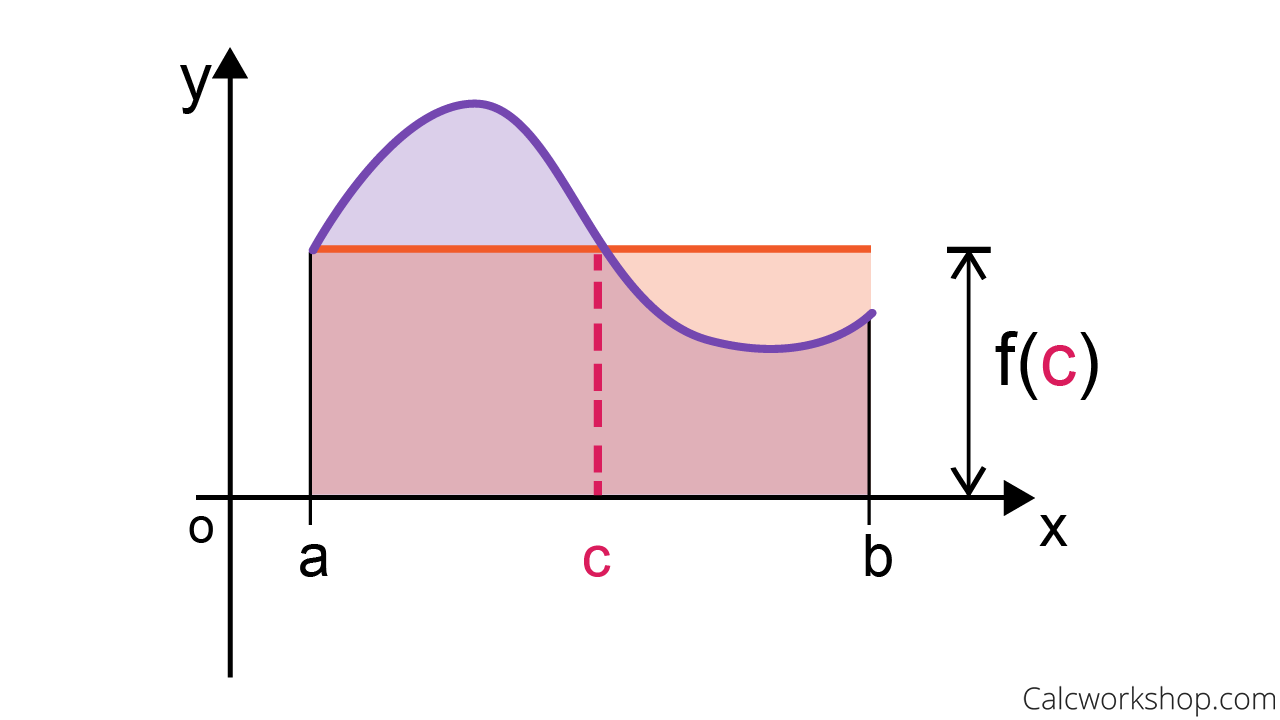
\includegraphics[scale=0.25]{mvt}
    \caption{Illustration for Mean Value Theorem for Integrals }
    \label{fig:mvt}
    \end{figure}
\vspace{0.5em}

By applying this exact theorem to our probability density function $p(x)$ over the interval $[i\Delta, (i+1)\Delta]$, we establish that there must exist a value $x_i$ inside each bin such that:
\begin{equation}
\int_{i\Delta}^{(i+1)\Delta} p(x) \, dx = p(x_i)\Delta
\end{equation}

We can now quantize the continuous variable $x$ by assigning any observed value to the representative point $x_i$ whenever $x$ falls within the $i$-th bin. Consequently, the discrete probability of observing the value $x_i$ is given by $p(x_i)\Delta$. Substituting this discrete distribution into the standard formulation of Shannon entropy yields:
\begin{equation}
H_\Delta = -\sum_{i} p(x_i)\Delta \ln \big( p(x_i)\Delta \big) = -\sum_{i} p(x_i)\Delta \ln p(x_i) - \ln \Delta
\end{equation}
where we have utilized the normalization property $\sum_{i} p(x_i)\Delta = 1$, which directly follows from the total area under the probability density curve.

To evaluate this expression in the continuous limit, we omit the coordinate-dependent scaling term $-\ln \Delta$ and consider the limiting behavior as the bin width approaches zero ($\Delta \to 0$). In this asymptotic limit, the discrete summation in the first term transforms directly into a Riemann integral, such that:
\begin{equation}
\lim_{\Delta \to 0} \left\{ -\sum_{i} p(x_i)\Delta \ln p(x_i) \right\} = -\int p(x) \ln p(x) \, dx
\end{equation}

The quantity on the right-hand side is defined as the \textbf{differential entropy}, denoted as:
\begin{equation}
H[x] = -\int p(x) \ln p(x) \, dx
\end{equation}

It is critical to observe that the discrete and continuous forms of entropy differ by the quantity $\ln \Delta$, which explicitly diverges as $\Delta \to 0$. This divergence reflects the underlying physical reality that specifying a continuous variable precisely down to an exact point requires an infinite amount of informational bits. For a multi-dimensional system defined over a vector of continuous variables $\mathbf{x}$, the total differential entropy is analogously given by:
\begin{equation}
H[\mathbf{x}] = -\int p(\mathbf{x}) \ln p(\mathbf{x}) \, d\mathbf{x}
\end{equation}
\subsection{Continuous Maximum Entropy}
To find the maximum entropy configuration for a continuous variable, we maximize the differential entropy subject to normalization, a fixed mean ($\mu$), and a fixed variance ($\sigma^2$):
\begin{align}
\int_{-\infty}^{\infty} p(x) \, dx &= 1 \\
\int_{-\infty}^{\infty} x p(x) \, dx &= \mu \\
\int_{-\infty}^{\infty} (x - \mu)^2 p(x) \, dx &= \sigma^2
\end{align}
Using the method of Lagrange multipliers, we construct the functional $\tilde{H}[p]$ with multipliers $\lambda_1$, $\lambda_2$, and $\lambda_3$:
\begin{align}
\tilde{H}[p] = -\int_{-\infty}^{\infty} p(x) \ln p(x) \, dx &+ \lambda_1 \left( \int_{-\infty}^{\infty} p(x) \, dx - 1 \right) \nonumber \\
&+ \lambda_2 \left( \int_{-\infty}^{\infty} x p(x) \, dx - \mu \right) \nonumber \\
&+ \lambda_3 \left( \int_{-\infty}^{\infty} (x - \mu)^2 p(x) \, dx - \sigma^2 \right)
\end{align}

By distributing the scalar multipliers inside the integration operators, we can collect the system variables under a single, unified continuous functional:
\begin{equation}
\tilde{H}[p] = \int_{-\infty}^{\infty} \Big[ -p(x) \ln p(x) + \lambda_1 p(x) + \lambda_2 x p(x) + \lambda_3 (x - \mu)^2 p(x) \Big] dx - \lambda_1 - \lambda_2\mu - \lambda_3\sigma^2
\end{equation}
Applying the calculus of variations, we take the functional derivative with respect to $p(x)$ and set it to zero:

\begin{equation}
\begin{aligned}
\frac{\partial \tilde{H}}{\partial p(x)}  =  -\ln p(x) - 1 + \lambda_1 + \lambda_2 x + \lambda_3 (x - \mu)^2 = 0 \\
\ln p(x) = -1 + \lambda_1 + \lambda_2 x + \lambda_3 (x - \mu)^2
\end{aligned}
\end{equation}
Isolating the density function $p(x)$ via exponentiation reveals its underlying mathematical architecture:
\begin{equation}
p(x) = \exp \left\{ -1 + \lambda_1 + \lambda_2 x + \lambda_3 (x - \mu)^2 \right\}
\end{equation}

To evaluate the multipliers, we substitute this form back into the initial constraints. Due to the required symmetry of the distribution around the mean $\mu$, the linear coefficient $\lambda_2$ is forced to $0$. The remaining exponential terms are split into a scaling constant and a functional component:
\begin{equation}
p(x) = \exp(-1 + \lambda_1) \cdot \exp\left\{\lambda_3 (x - \mu)^2\right\}
\end{equation}

Solving the remaining definite Gaussian integrals under the normalization and variance constraints yields $\lambda_3 = -1/(2\sigma^2)$ and $\exp(-1 + \lambda_1) = 1/(2\pi\sigma^2)^{1/2}$, leading directly to the definitive Gaussian density function:
\begin{equation}
p(x) = \frac{1}{(2\pi\sigma^2)^{1/2}} \exp \left\{ -\frac{(x - \mu)^2}{2\sigma^2} \right\}
\end{equation}

Substituting this profile back into the differential entropy integral yields the maximum attainable uncertainty value for a continuous variable with known variance:
\begin{equation}
H[x] = \frac{1}{2} \left\{ 1 + \ln(2\pi\sigma^2) \right\}
\end{equation}

\section{Kullback-Leibler Divergence}
It is a measure of how much one probability distribution diverges from the second, reference probability distribution. It is often thought of a distance between two distributions. 
\begin{equation}
D_{KL} = H(p,q) - H(p)
\end{equation}
We know that the entropy of a distribution X is :
\begin{equation}
H(X) = -\int_{-\infty}^{\infty} f(x) \log f(x) \, dx
\end{equation}
so it can be written as 
\begin{equation}
D_{KL} = - \int p(x) \ln(q(x)) \, dx - \left( - \int p(x) \ln(p(x)) \, dx \right)
\end{equation}
\begin{equation}
D_{KL} = -\int p(x) \ln{\frac{q(x)}{p(x)}} \, dx
\end{equation}
\section{Conditional Entropy}
Considering a joint distribution between two set of variables $x$ and $y$; if a value of $x$ is already known, the additional information needed to specify the corresponding value of y can be given as $- \ln(p(y|x)) \ $. Thus the average additional information needed to specify $y$ can be written as

\begin{equation}
H[y|x] = - \int \int p(y,x) \ln p(y|x) \, dy dx
\end{equation}
Joint entropy can be written as :
\begin{equation}
H[x,y] = - \int \int p(x,y) \ln(p(x,y)) \, dy dx
\end{equation}
using product rule  $p(x,y) = p(y|x)p(x)$
\begin{equation}
H[x,y] = - \int \int p(x,y) \ln(p(y|x)p(x)) \, dy dx
\end{equation}
\begin{equation}
H[x,y] = - \int \int p(x,y) \ln(p(y|x)) \, dy dx - \int \int p(x,y) \ln(p(x)) \, dy dx
\end{equation}
From here we can see that the first part is equals to  $H[y|x] = - \int \int p(x,y) \ln(p(y|x))$  and the second part is not dependent on y so we can rearrange it as following 
\begin{equation}
- \int \int p(x,y) \ln(p(x))\, dy dx
\end{equation}
\begin{equation}
= - \int \left( \int p(x,y) \, dy \right) \ln(p(x)) \, dx
\end{equation}
as it is taking all possible values of y so it will be 
\begin{equation}
= - \int p(x) \ln(p(x)) \, dx = H[x]
\end{equation}
So it can be said that, 
\begin{center}
\textcolor{red}{ $H[x,y] = H[y|x] + H[x]$}
\end{center}
\section{Mutual Entropy}
It measures how much information of one random variable shares with other. If two distribution are independent then $p(x,y) = p(x)p(y)$. So if we find the divergence then if it is 0 then it is independent. So we can calculate it by finding the divergence between the joint distribution and the product of the separate distributions. Then :
\begin{equation}
I(x,y) = D_{KL}\left( p(x,y) || p(x)p(y) \right)
\end{equation}
\begin{equation}
= - \int \int p(x,y) \ln\left( \frac{p(x)p(y)}{p(x,y)} \right) \, dx dy
\end{equation}
now if we expand the fraction 
\begin{equation}
= - \int \int p(x,y) \ln\left( \frac{p(x)}{p(x,y)} \right) \, dx dy  - \int \int p(x,y) \ln\left( \frac{p(y)}{p(x,y)} \right) \, dx dy
\end{equation}

Here we have two options comparing with respect to $x$ and $y$, considering one term will cancel out the other part. Lets take for $x$

\begin{equation}
= - \int \int p(x,y) \ln\left(p(x) \right) \, dx dy  - \int \int p(x,y) \ln\left( p(x,y) \right) \, dx dy
\end{equation}
\begin{equation}
= H[x] - H[x,y]
\end{equation}
Similarly we can do it for $y$ also :
So the equation will be 
\begin{equation}
I(x,y) = H[x] - H[x,y] = H[y] - H[x,y]
\end{equation}
\end{document}